\documentclass[a4paper, 12pt]{article}
\usepackage{pgfplots, mathtools}

%% Listings With Code-Styling and Grey Background
\usepackage{float, listings} 
\lstset{						% Global Listing settings
	language=Verilog,
	numbers=left,
	numberstyle=\tiny\color{gray},
%	firstnumber=1,
	numberfirstline=true,
	stepnumber=1,
	tabsize=2,
	breaklines=true,
}
\usepackage{xcolor, mdframed, graphicx}
\definecolor{code-gray}{gray}{0.93}

%% Make specific pages landscale for larger figures
\usepackage{pdflscape}

%% Custom FSM's
\usepackage{tikz}
\usetikzlibrary{automata, positioning, arrows}
\tikzset{very thick, ->, >=stealth', node distance=6cm, every state/.style={thick, fill=gray!10}, initial text=$ $}

%% Automatic Word Formatting
\usepackage{xspace}
\newcommand*{\Vivado}{\textit{Vivado}\xspace} % Italicize Vivado
\newcommand*{\SV}{\textbf{SystemVerilog}\xspace} % Bold SystemVerilog

%% Clickable links in the output PDF
\usepackage{hyperref}
\hypersetup{colorlinks=true, linktoc=all, linkcolor=black}

%% Figure Numbering Within Sections
\let\counterwithout\relax
\let\counterwithin\relax
\usepackage{chngcntr}
\counterwithin{figure}{section}

%% Macros for logic timing diagrams
\newcounter{wavenum}
\setlength{\unitlength}{1cm}
% advance clock one cycle, not to be called directly
\newcommand*{\clki}{
  \draw (t_cur) -- ++(0,.3) -- ++(.5,0) -- ++(0,-.6) -- ++(.5,0) -- ++(0,.3)
    node[time] (t_cur) {};
}
\newcommand*{\bitvector}[3]{
  \draw[fill=#3] (t_cur) -- ++( .1, .3) -- ++(#2-.2,0) -- ++(.1, -.3)
                         -- ++(-.1,-.3) -- ++(.2-#2,0) -- cycle;
  \path (t_cur) -- node[anchor=mid] {#1} ++(#2,0) node[time] (t_cur) {};
}
% \known{val}{length}
\newcommand*{\known}[2]{
    \bitvector{#1}{#2}{white}
}
% \unknown{length}
\newcommand*{\unknown}[2][XXX]{
    \bitvector{#1}{#2}{black!20}
}
% \bit{1 or 0}{length}
\newcommand*{\bit}[2]{
  \draw (t_cur) -- ++(0,.6*#1-.3) -- ++(#2,0) -- ++(0,.3-.6*#1)
    node[time] (t_cur) {};
}
% \unknownbit{length}
\newcommand*{\unknownbit}[1]{
  \draw[ultra thick,black!50] (t_cur) -- ++(#1,0) node[time] (t_cur) {};
}
% \nextwave{name}
\newcommand{\nextwave}[1]{
  \path (0,\value{wavenum}) node[left] {#1} node[time] (t_cur) {};
  \addtocounter{wavenum}{-1}
}
% \clk{name}{period}
\newcommand{\clk}[2]{
    \nextwave{#1}
    \FPeval{\res}{(\wavewidth+1)/#2}
    \FPeval{\reshalf}{#2/2}
    \foreach \t in {1,2,...,\res}{
        \bit{\reshalf}{1}
        \bit{\reshalf}{0}
    }
}

% \begin{wave}[clkname]{num_waves}{clock_cycles}
\newenvironment{wave}[3][clk]{
  \begin{tikzpicture}[draw=black, yscale=.7,xscale=1]
    \tikzstyle{time}=[coordinate]
    \setlength{\unitlength}{1cm}
    \def\wavewidth{#3}
    \setcounter{wavenum}{0}
    \nextwave{#1}
    \foreach \t in {0,1,...,\wavewidth}{
      \draw[dotted] (t_cur) +(0,.5) node[above] {t=\t} -- ++(0,.4-#2);
      \clki
    }
}{\end{tikzpicture}}

%$ Specific Line Breaks
% See https://tex.stackexchange.com/questions/26174/ for details
\usepackage[british]{babel} 

%% Page Margins
\usepackage[margin=1.00in]{geometry}

%% Beginning of Document
\begin{document}
\counterwithin{lstlisting}{section} % Listings are numbered within sections
% Title
\title{ECE 440 - Project \#8}
\author{Collin Heist}
\date{\today}
\maketitle

% Table of Content and Listings
\pagenumbering{roman}
\tableofcontents
\renewcommand{\listfigurename}{Figures}
\listoffigures
\lstlistoflistings
\newpage
\pagenumbering{arabic}

% Beginning of Report
\section{Design}
\subsection{Codon Reader}
I chose to implement this project with two relatively complicated modules (although in hindsight, I should have partitioned my project more). The first one being the codon-reading module, that is responsible for reading the codon memory and storing the parsed codons for later operations. The FSM I designed for this module is shown in \textbf{Figure~\ref{fig:fsm-codon-reader}}.

\begin{figure}[H]
\centering
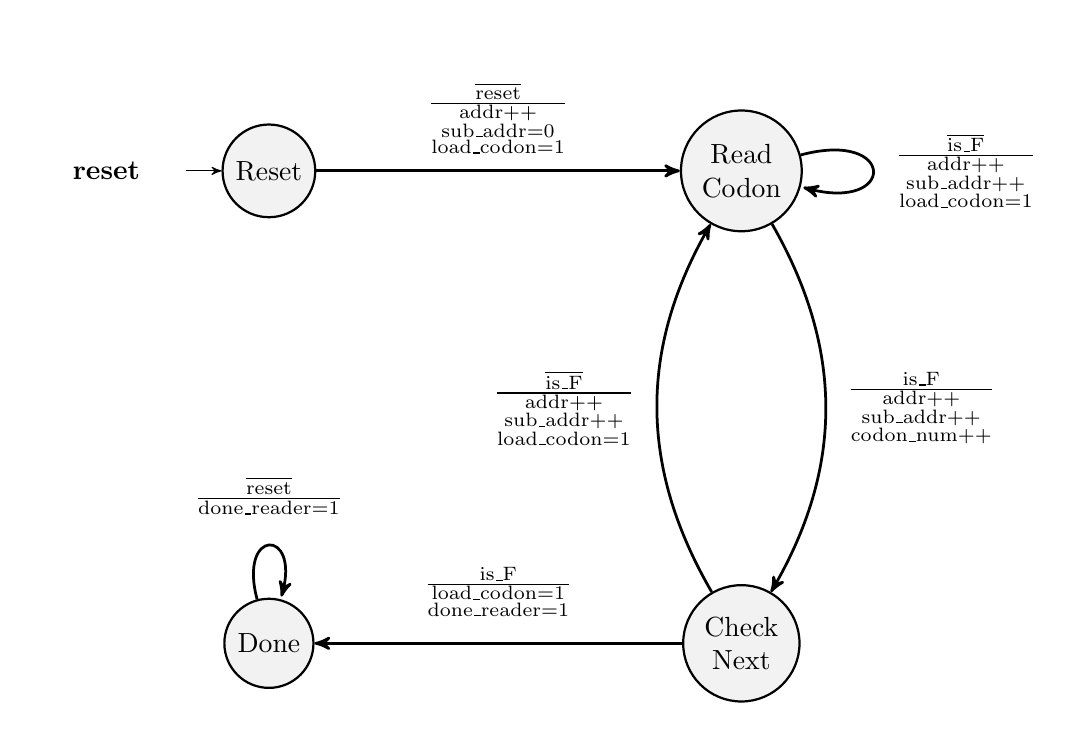
\begin{tikzpicture}[initial text=\textbf{reset}, every node/.style={circle, minimum size=2cm, align=center}]
	\node[initial, state] (Reset) {Reset};
	\node[state, right of=Reset] (Read Codon) {Read\\ Codon};
	\node[state, below of=Read Codon] (Check Next) {Check\\ Next};
	\node[state, below of=Reset] (Done) {Done};
	\draw[->, line width=0.35mm]
		(Reset) edge[above] node[yshift=-0.5cm]{$\frac{\overline{\text{reset}}}{\substack{\text{addr++}\\ \text{sub\_addr=0}\\ \text{load\_codon=1}}}$} (Read Codon)
		(Read Codon) edge[loop right] node{$\frac{\overline{\text{is\_F}}}{\substack{\text{addr++}\\ \text{sub\_addr++}\\ \text{load\_codon=1}}}$} (Read Codon)
		(Read Codon) edge[bend left, right] node{$\frac{\text{is\_F}}{\substack{\text{addr++}\\ \text{sub\_addr++}\\ \text{codon\_num++}}}$} (Check Next)
		(Check Next) edge[bend left, left] node{$\frac{\overline{\text{is\_F}}}{\substack{\text{addr++} \\ \text{sub\_addr++} \\ \text{load\_codon=1}}}$} (Read Codon)
		(Check Next) edge[above] node[yshift=-0.5cm]{$\frac{\text{is\_F}}{\substack{\text{load\_codon=1}\\ \text{done\_reader=1}}}$} (Done)
		(Done) edge[loop above] node[yshift=-0.5cm]{$\frac{\overline{\text{reset}}}{\text{done\_reader=1}}$} (Done);
\end{tikzpicture}
\caption{Codon Reading Finite State Machine}
\label{fig:fsm-codon-reader}
\end{figure}

As evident by the FSM, this is a fairly straightforward module. The codon memory is instantiated, and then each sequential memory location is read, filling in a 3D array (called \textbf{codons}) as it goes. Whenever an \textbf{0xF} is detected--that value is skipped, \textbf{codon\_num} is incremented (signifying which codon we are \textit{filling}) and the process repeats. This is repeated until two sequential \textbf{0xF}'s are detected, at which point the \textbf{done} state is entered, and the process switches to entirely combinational logic. 

The combinational logic in this module is fairly substantial, handling all of the codon-subindex output, and \textit{end of codon} detection. This module takes in a 3-bit signal called \textbf{codon\_index} which signifies which 4-bit nibble of all codons to look at (for example, nibble 1 of codon \textbf{0x16A2} would be \textbf{0x6}). Nibbles of all codons (1-5) are output at all times through signals \textbf{codonX}. The most important part (with regards to counting codons used in the next module) is the end of codon detection. To aid in this, the codon memory is created with one extra nibble per codon (so they are all technically 6 nibbles long), and the entire memory is initialized with 1's. Then, a 5-bit (one bit for each codon) output \textbf{end\_of\_codon} looks at the \textit{next} nibble of all codons (so \textbf{codon\_index}+1) to see if that contains \textbf{0xF}, signifying the current nibble is the last one in memory.

\subsection{Codon Counter}
The second module created for this project is the codon counter. This is fairly substantial, and should have probably been done in two or more separate modules. This module waits for the reader module to finish reading (signified by \textbf{done\_reader} going high), and then it starts going through the gene memory, counting instances of each codon. The FSM for this is shown below in \textbf{Figure~\ref{fig:fsm-codon-counter}}.

\begin{figure}[H]
\centering
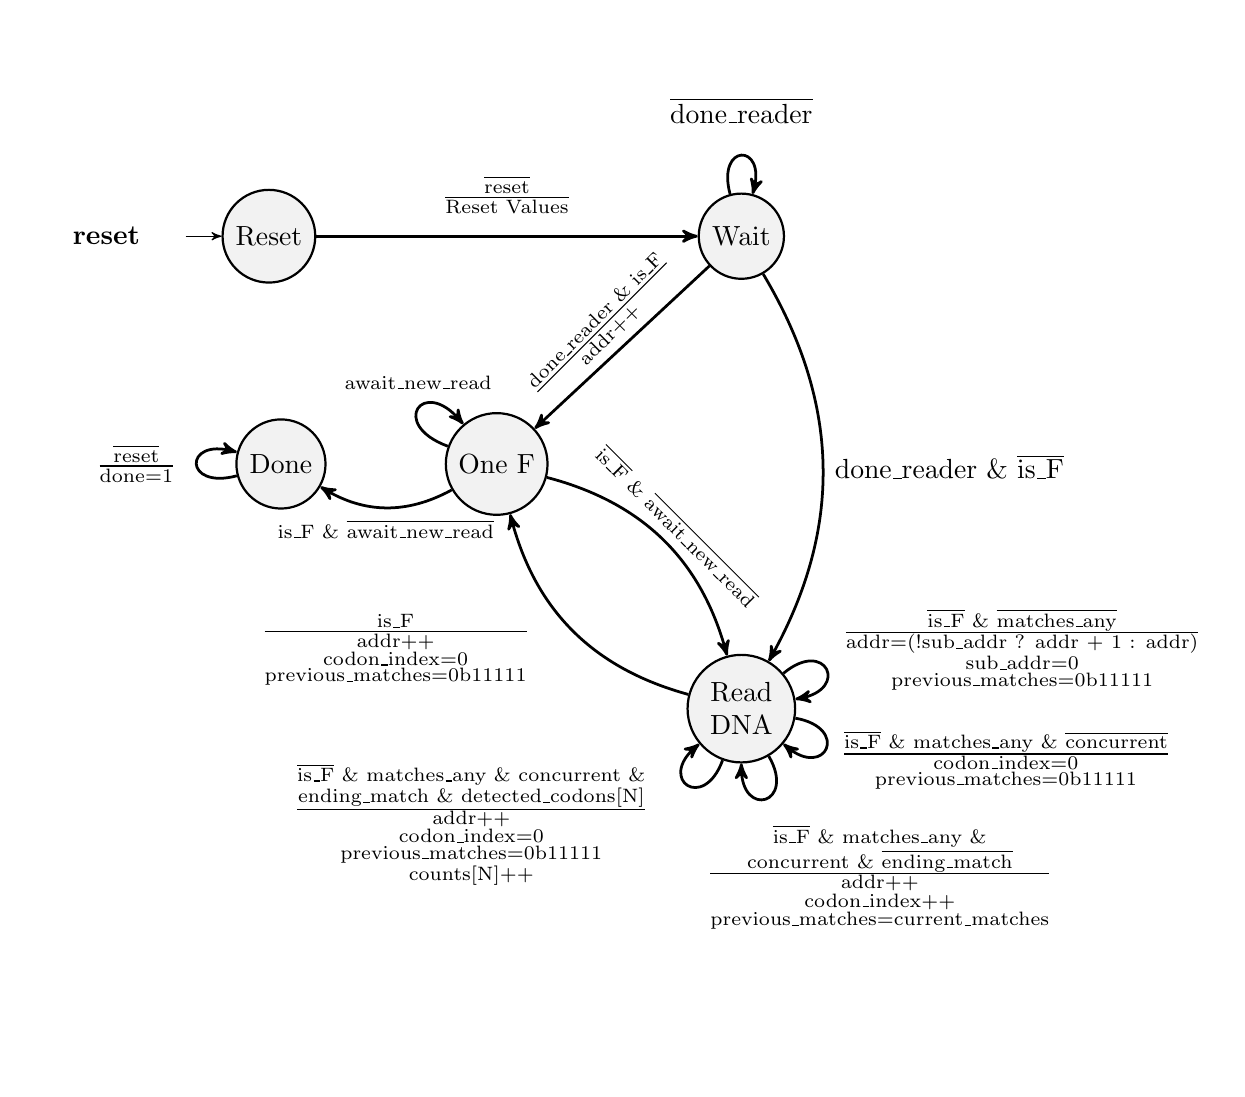
\begin{tikzpicture}[initial text=\textbf{reset}, every node/.style={circle, minimum size=2cm, align=center}]
	\node[initial, state] (Reset) {Reset};
	\node[state, right of=Reset] (Wait) {Wait};
	\node[state, below right=2cm and 2cm of Reset] (One F) {One F};
	\node[state, below of=Wait] (Read DNA) {Read\\ DNA};
	\node[state, left=1.5cm of One F] (Done) {Done};
	\draw[->, line width=0.35mm]
		(Reset) edge[above] node[yshift=-.5cm]{$\frac{\overline{\text{reset}}}{\text{Reset Values}}$} (Wait)
		(Wait) edge[loop above, looseness=6] node[yshift=-.5cm]{$\overline{\text{done\_reader}}$} (Wait)
		(Wait) edge[above left] node[anchor=center, rotate=45, yshift=0.35cm]{$\frac{\text{done\_reader \& is\_F}}{\text{addr++}}$} (One F)
		(Wait) edge[bend left, right] node[]{done\_reader \& $\overline{\text{is\_F}}$} (Read DNA)
		(One F) edge[loop, out=160, in=130, above, looseness=6] node[yshift=-.75cm]{\scriptsize{await\_new\_read}} (One F)
		(One F) edge[bend left, below] node[yshift=1.25cm]{\scriptsize{is\_F \& $\overline{\text{await\_new\_read}}$}} (Done)
		(One F) edge[bend left, above right] node[anchor=center, rotate=-45, yshift=.25cm]{\scriptsize{$\overline{\text{is\_F}}$ \& $\overline{\text{await\_new\_read}}$}} (Read DNA)
		(Done) edge[loop left, looseness=6] node[xshift=.25cm]{$\frac{\overline{\text{reset}}}{\text{done=1}}$} (Done)
		(Read DNA) edge[bend left, left] node[anchor=center, xshift=-2.25cm, yshift=-.25cm]{$\frac{\text{is\_F}}{\substack{\text{addr++}\\ \text{codon\_index=0}\\ \text{previous\_matches=0b11111}}}$} (One F)
		(Read DNA) edge[loop, out=40, in=10, looseness=5, right] node[xshift=0cm, yshift=0.25cm]{$\frac{\overline{\text{is\_F}}\text{ \& }\overline{\text{matches\_any}}}{\substack{\text{addr=(!sub\_addr ? addr + 1 : addr)}\\ \text{sub\_addr=0}\\ \text{previous\_matches=0b11111}}}$} (Read DNA)
		(Read DNA) edge[loop, out=-10, in=-40, looseness=5, right] node[yshift=-0.15cm]{$\frac{\overline{\text{is\_F}}\text{ \& }\text{matches\_any \& }\overline{\text{concurrent}}}{\substack{\text{codon\_index=0}\\ \text{previous\_matches=0b11111}}}$} (Read DNA)
		(Read DNA) edge[loop, out=-60, in=-90, looseness=5, right] node[xshift=-1cm, yshift=-1cm]{$\frac{\substack{\overline{\text{is\_F}}\text{ \& }\text{matches\_any \&}\\ \text{concurrent \& }\overline{\text{ending\_match}}}}{\substack{\text{addr++}\\ \text{codon\_index++}\\ \text{previous\_matches=current\_matches}}}$} (Read DNA)
		(Read DNA) edge[loop, out=-110, in=-140, looseness=5, left] node[anchor=center, xshift=-2.75cm, yshift=-0.5cm]{$\frac{\substack{\overline{\text{is\_F}}\text{ \& matches\_any \& concurrent \&}\\ \text{ending\_match \& detected\_codons[N]}}}{\substack{\text{addr++}\\ \text{codon\_index=0}\\ \text{previous\_matches=0b11111}\\ \text{counts[N]++}}}$} (Read DNA);
\end{tikzpicture}
\caption{Codon Counter Finite State Machine}
\label{fig:fsm-codon-counter}
\end{figure}

When reset is no longer asserted, the values used in this module are reset. The notable one here is that \textbf{previous\_matches} is reset to \textbf{0b11111} as opposed to zeros. This is done so that during the detection of full codons, single-nibble codons are detected (I'll go into more detail later). I could technically remove the \textbf{Wait} state by and-ing \textbf{reset} and \textbf{done\_reader} to start the FSM. However, as soon as the codon reading is finished, the gene memory is read. Not shown in the FSM (at least on the \textbf{Read DNA} state) is the relevance of \textbf{await\_new\_read}. This is a signal used to account for the one clock delay in all reads, and is toggled during every clock cycle while in the \textbf{Read DNA} and \textbf{One F} states.

The internal control signals being used for most of this logic are the \textbf{is\_F}, \textbf{matches\_any}, \textbf{concurrent\_matches} (labeled concurrent), \textbf{ending\_match}, and \textbf{detected\_codons}.Their assignments are shown in \textbf{Listing~\ref{lst:control-signals}}.

\begin{mdframed}[backgroundcolor=code-gray, roundcorner=10pt, innerleftmargin=25, innertopmargin=5, innerbottommargin=5]	
\begin{lstlisting}[nolol=True, caption=Internal Logic Signal Assignment, label={lst:control-signals}, language=Verilog]
always_comb begin : codon_match_detection
	current_matches[0] = ((memory_out == codon1) && (codon1 != 4'hF));
	current_matches[1] = ((memory_out == codon2) && (codon2 != 4'hF));
	current_matches[2] = ((memory_out == codon3) && (codon3 != 4'hF));
	current_matches[3] = ((memory_out == codon4) && (codon4 != 4'hF));
	current_matches[4] = ((memory_out == codon5) && (codon5 != 4'hF));

	ending_match = | (current_matches & end_of_codon);
	concurrent_matches = | (current_matches & previous_matches);
	matches_any = | current_matches;	
	detected_codons = (current_matches & previous_matches & end_of_codon);
end : codon_match_detection
\end{lstlisting}
\end{mdframed}

Although the \textbf{Read DNA} state looks complicated, it really only handles five conditions. These five conditions, and the action taken, are as follows:

\begin{itemize}
\item The current gene nibble is \textbf{0xF}-- move to the \textbf{One F} state.
\item No matches on the current gene to any of the codons, shown by $\overline{\text{matches\_any}}$ -- increment the address only if we were looking at the start nibble of all codons, otherwise return to the start codon index.
\item There was a match, but not a concurrent one -- don't increment the address, restart on the first nibble of all codons.
\item There is a concurrent match, but not an end-of-codon one -- store the current matches, go to the next codon index and address.
\item There's an ending, concurrent match on codon[\textbf{N}] (1-5) -- increment that codon's count, reset the codon index and previous match values, and finally go to the next address.
\end{itemize}

\subsection{Hardware Wrapper}
The final \textit{module} I wrote was the hardware wrapper -- it takes the clock, reset, switches, and LED inputs and takes care of the output LED assignment. There is nothing of note here, however I was unable to implement the \textbf{.xdc} file portion of this project because I couldn't access the lab and was unable to run \Vivado on my computer.

\section{Tribulations}
\label{sec:tribulations}
I initially planned on having all bits of all codons as inputs to the codon counting module, but I realized after beginning that design process that this would require at least 100-bits of input to the module \textit{just for the codons}, at that seemed quite \textit{messy}. Although this is not a direct problem, it did require a redesign, and I ended up implementing the nibble-indexing (with \textbf{codon\_index}) instead.

I initially did not account for the one clock cycle delay on reading from the gene memory, and the first instance of \textbf{0xF} would terminate the counting. Because it would be \textbf{0xF} on the first cycle, and had not yet updated by the time it was evaluated for the \textbf{One F} state. I fixed this by adding the \textbf{await\_new\_read} signal.

\begin{landscape}
\section{Simulations}
I was also unable to perform any simulations with the synthesized design (however I did verify it synthesized without error) -- but the behavioral simulation went as expected, and the last few cycles of the codon reader are shown below in \textbf{Figure~\ref{fig:behav-codon-reader}}.

\begin{figure}[H]
\centering
\includegraphics[width=0.85\paperheight, keepaspectratio=true]{Sources/codon_reader.PNG}
\caption{Codon Reader Behavioral Simulation.}
\label{fig:behav-codon-reader}
\end{figure}

This simulation was performed on the example codon and gene memory instance, and viewing \textbf{Codons} shows how the loading sequence works. All stored codons start off as \textbf{0xFFFFFF}, and are loaded sequentially (shown in reverse order in the simulation, for some reason). After two sequential instances of \textbf{0xF}, the done signal is asserted. I also have an  image of the final count outputs, shown in \textbf{Figure~\ref{fig:behav-count-leds}}.

\begin{figure}[H]
\centering
\includegraphics[width=0.85\paperheight, keepaspectratio=true]{Sources/switch_outputs.png}
\caption{All codon counts asserted on the LEDs.}
\label{fig:behav-count-leds}
\end{figure}

When the switches are 0, \textbf{LED0} goes high as soon as the counting is done, and then the sequence of switches cycles through the counts of each codon.
\end{landscape}

\section{Source Code}
\begin{mdframed}[backgroundcolor=code-gray, roundcorner=10pt, innerleftmargin=25, innertopmargin=5, innerbottommargin=5]	
\lstinputlisting[caption=Codon Reader Module, label={lst:codon-reader}]{Sources/codon_reader.sv}
\end{mdframed}

\begin{mdframed}[backgroundcolor=code-gray, roundcorner=10pt, innerleftmargin=25, innertopmargin=5, innerbottommargin=5]	
\lstinputlisting[caption=Codon Counter Module, label={lst:codon-counter}]{Sources/codon_counter.sv}
\end{mdframed}

\begin{mdframed}[backgroundcolor=code-gray, roundcorner=10pt, innerleftmargin=25, innertopmargin=5, innerbottommargin=5]	
\lstinputlisting[caption=Hardware Wrapper, label={lst:hardware-wrapper}]{Sources/hardware_wrapper.sv}
\end{mdframed}

\begin{mdframed}[backgroundcolor=code-gray, roundcorner=10pt, innerleftmargin=25, innertopmargin=5, innerbottommargin=5]	
\lstinputlisting[caption=Simulation Testbench, label={lst:testbench}]{Sources/testbench.sv}
\end{mdframed}

\end{document}